\documentclass[journal]{IEEEtran}

\usepackage{cite}
\usepackage{amsmath,amssymb,amsfonts}
\usepackage{graphicx}
\usepackage{textcomp}
\usepackage{xcolor}
\usepackage{booktabs}
\usepackage{multirow}
\usepackage{url}

\title{Exact-Quota Mixed-Precision FIR Coefficient\\
Quantization: Dynamic Programming, FPGA Validation,\\
and Feasibility Analysis of Response-Aware Allocation}

\author{Ruirui Bai%
\thanks{Ruirui Bai is with Shanxi University, Taiyuan, China (e-mail: bairuirui0924@163.com).}}

\begin{document}
\maketitle

\begin{abstract}
This technical report documents the design, analysis, and experimental
evaluation of exact-quota mixed-precision coefficient quantization for
FIR filters. The central problem assigns each of $N$ fixed coefficients
one of three binary widths---16-bit, 8-bit, or 4-bit---subject to exact
count constraints, and minimizes the total squared coefficient
quantization error. This is equivalent to a unit-capacity bipartite
transportation problem, a fact that limits the algorithmic novelty
claim: the dynamic programming (DP) solution presented here is a
structure-specific realization of a known cost-constrained DP class,
not a new optimization principle.

The report documents validation across three levels: (1) software---29
exhaustive consistency checks, 108 test configurations comparing DP,
greedy, and MILP baselines; (2) FPGA---6 synthesis/route experiments
for an 8-tap filter on Xilinx Artix-7, and 4 synthesis/route
experiments for a 48-tap symmetric-folded filter; (3) physical
hardware---942 bit-exact functional comparisons across three
configurations on an ACX750 development board. A 48-tap robustness
study covers 15 design/quota combinations from 5 filter specifications;
DP meets a $-40$\,dB stopband limit in 2 of 15 cases, greedy in 0.
A response-aware allocation branch was explored; a 48-tap binary-product
MILP reformulation was manually stopped after about 93 seconds because
its root relaxation showed negligible progress toward proving optimality.
The run returned no solver exit flag or final allocation, and the branch
was closed under the pre-declared slow-progress stopping condition. All
negative results are reported.
No novelty claim is made.
\end{abstract}

\begin{IEEEkeywords}
FIR filter, coefficient quantization, dynamic programming,
mixed-precision, FPGA, assignment problem.
\end{IEEEkeywords}

\section{Introduction}

Finite-word-length implementation of FIR filters requires assigning a
coefficient precision to each tap. When the available hardware supports
a discrete set of widths---for example, 16-bit, 8-bit, and 4-bit
multipliers---and the system specifies exact counts at each width, the
assignment becomes a combinatorial optimization problem. The natural
objective in coefficient-domain design is to minimize the total squared
coefficient quantization error.

This report studies the exact-quota version of that problem: given
$N$ tap coefficients and integer counts $n_{16}$, $n_8$, $n_4$ with
$n_{16}+n_8+n_4=N$, assign each coefficient a width from
$\{16,8,4\}$ to minimize
\begin{equation}
\min_{\mathbf{w}} \sum_{i=1}^{N} \bigl(h_i - Q(h_i,w_i)\bigr)^2
\label{eq:sse}
\end{equation}
subject to $|\{i: w_i=w\}|=n_w$ for each width~$w$.

A DP recurrence processes coefficients in order and achieves the global
minimum for~\eqref{eq:sse}. The formulation is equivalent to a
unit-capacity bipartite transportation problem or binary assignment
MILP, a relationship established in Section~\ref{sec:formulation}
and verified empirically in Section~\ref{sec:validation}.

The report is organized as follows. Section~\ref{sec:related}
reviews related work including the closest prior formulations.
Section~\ref{sec:formulation} states the problem and its equivalences.
Section~\ref{sec:algorithm} describes the DP and greedy algorithm.
Section~\ref{sec:validation} reports software validation.
Section~\ref{sec:fpga} describes the FPGA case studies.
Section~\ref{sec:robustness} reports the robustness study.
Section~\ref{sec:response_aware} documents the response-aware
allocation investigation and its negative result.
Section~\ref{sec:conclusion} concludes.

\section{Related Work}
\label{sec:related}

% Related work section for tech report

Several lines of prior work are directly relevant. Twelve papers were
reviewed in full in the project literature assessment, and six additional
works received abstract-level screening. The reviewed set is targeted,
not an exhaustive search of the field.

\subsection{Finite-Word-Length FIR Design}

Kodek and Steiglitz~\cite{kodek1980filter} analyzed length-wordlength
tradeoffs for FIR filters, proving a nonzero lower bound on weighted
Chebyshev error for fixed coefficient wordlength. Their complexity proxy
$Nb$ motivates joint optimization; their analysis assumes a common
wordlength, not per-coefficient quotas.

Lim, Parker, and Constantinides~\cite{lim1982finite} minimized FIR
designs over discrete coefficient-value spaces using integer linear and
quadratic programming, comparing discrete-space designs with rounded
infinite-wordlength designs. Lim~\cite{lim1990nprm} extended this to
normalized peak-ripple minimization, using MILP methods with passband
gain as a design variable.

\subsection{SPT-Based and Hardware-Aware Coefficient Allocation}

Several methods allocate signed-power-of-two (SPT) terms across
coefficients. Llorens, Hadjicostis, and Ni~\cite{llorens2005integercost}
formulated FIR coefficient quantization under a scalar total integer-cost
constraint using a constrained-shortest-path DP. Their alpha=2 case
relates coefficient-vector error to frequency-response MSE via Parseval's
theorem. For exact three-width quotas, a radix encoding
($r_{16}=B+1$, $r_8=2$, $r_4=1$, $B=N+1$) reduces the quota DP to a
scalar exact-cost DP, so the present quota DP is a specialized
realization of Llorens et al.'s framework, not a new optimization class.
They also describe a greedy algorithm with a conditional optimality
guarantee: the guarantee depends on the marginal error reduction as the
integer cost increases. The sparse costs used in the radix encoding do not
automatically satisfy that condition: intermediate cost levels represent no
additional width choice, while the final jump to 16 bits can have a positive
error reduction. The greedy baseline in this report instead selects the
largest immediate squared-error reduction among quota-feasible 4-to-8 and
8-to-16 upgrades. It is a comparator only; no optimality guarantee is
claimed, and it is not identified with Llorens et al.'s conditionally
optimal greedy algorithm.

Chen and Willson~\cite{chen1999trellis} used a trellis (Viterbi-like)
search for SPT term allocation against frequency-response criteria; their
survivor pruning does not guarantee global optimality. Li, Lim, Lian,
and Song~\cite{li2002polynomial} allocated a global SPT-term budget with
variable per-coefficient counts using greedy sequential allocation;
the authors describe the result as suboptimal.

Aktan, Yurdakul, and D\"{u}ndar~\cite{aktan2008algorithm} used
branch-and-bound (FIRGAM) with LP for coefficient bounds to reduce SPT
count while meeting frequency specifications; worst-case runtime is
exponential.

Kuo, Lin, and Liu~\cite{kuo2011complexity} integrated successive SPT
allocation with common-subexpression elimination under an exact global
post-CSE addition budget, reporting 0.35-$\mu$m CMOS synthesis results.

\subsection{Subexpression-Space and Structure Optimization}

Yu and Lim~\cite{yu2007subexpression} optimized FIR coefficients
directly in a discrete subexpression space using branch-and-bound MILP,
minimizing frequency-response ripple subject to an adder budget. This is
a direct coefficient-space search, not a two-stage quantize-then-CSE
pipeline.

Blad and Gustafsson~\cite{blad2010integer} used ILP to optimize
partial-product reduction trees and pipeline registers for fixed
coefficient representations, targeting 90-nm CMOS. Their decision
variables are hardware structural elements, not coefficient widths.

\subsection{Mixed-Precision FIR Allocation}

Fang, Chen, Chen, Wang, and You~\cite{fang2025mixedprecision} proposed a
PSO-based bit-allocation framework applied to FIR filter design with a
frequency-domain minimax objective and aggregate bit-consumption
constraint. Their constraint is an inequality on total bits ($\sum b_n
\le N \bar{b}$), not exact per-width counts. Their allocation assumes
symmetric widths (linear-phase structure). This is the closest prior
mixed-precision FIR allocation paper; it differs from the present work
in constraint type, objective, and solution method.

Sarma, Sai, and Chatterjee~\cite{sarma2026coefficient} used a
coefficient-magnitude threshold to select exact or LUT-approximate
multipliers under an output-error budget on a Zynq UltraScale+ radar DDC
implementation. Their quantization model (approximate arithmetic)
differs from fixed-point coefficient widths.

\subsection{Neural-Network Mixed-Precision}

Yang and Jin's FracBits~\cite{yang2021fracbits} assigns fractional
bit-widths in neural-network quantization. It is included as
methodological context; it is not a direct FIR baseline.


\section{Problem Formulation}
\label{sec:formulation}

% Problem formulation section for tech report

\subsection{Exact-Quota Width Assignment}

Let $\mathbf{h} = [h_1, \ldots, h_N]$ be a fixed real-valued FIR
coefficient vector and let $\mathcal{W} = \{16, 8, 4\}$ be the set of
allowed binary widths. Given integer quotas $n_{16}$, $n_8$, $n_4$ with
$n_{16}+n_8+n_4=N$, the problem is to find the width assignment
$\mathbf{w} \in \mathcal{W}^N$ minimizing~\eqref{eq:sse} subject to
\begin{equation}
|\{i : w_i = w\}| = n_w, \quad w \in \mathcal{W}.
\label{eq:quota}
\end{equation}
The quantization operator $Q(h,w)$ rounds $h$ to the nearest value
representable with $w$ bits (1 sign, $w-1$ fractional bits, no saturation
within the tested range).

\subsection{Equivalence to Unit-Capacity Transportation}

Problem~\eqref{eq:sse}--\eqref{eq:quota} is a binary assignment MILP.
Let $x_{i,k} \in \{0,1\}$ indicate that coefficient $i$ receives width
$\text{choices}(k)$; the cost of assignment $x_{i,k}=1$ is
$c_{i,k} = (h_i - Q(h_i, \text{choices}(k)))^2$. Then:
\begin{align}
\min_{\mathbf{x}} \quad & \sum_{i=1}^N \sum_{k=1}^3 c_{i,k} x_{i,k}
\label{eq:milp_obj}\\
\text{s.t.} \quad
& \sum_k x_{i,k} = 1, \quad i=1,\ldots,N \label{eq:milp_assign}\\
& \sum_i x_{i,k} = n_k, \quad k=1,2,3 \label{eq:milp_quota}\\
& x_{i,k} \in \{0,1\} \label{eq:milp_binary}
\end{align}
is a unit-capacity bipartite transportation / min-cost flow problem. The
network has a source connected to each of the $N$ coefficient nodes
(capacity 1, cost 0), each coefficient node connected to each of the 3
width nodes (capacity 1, cost $c_{i,k}$), and each width node connected
to a sink (capacity $n_k$, cost 0). Sending $N$ units of flow minimizes
total cost and satisfies all quotas exactly.

The LP relaxation obtained by replacing $x_{i,k}\in\{0,1\}$ with
$x_{i,k}\geq 0$ has integral extreme points: after multiplying one
partition of constraint rows by $-1$, its constraint matrix is a directed
bipartite node--arc incidence matrix and is totally unimodular. Since the
assignment and quota right-hand sides are integers, an optimal LP extreme
point is integral. Thus the assignment formulation can also be solved as a
linear program; the reported MILP runs are implementation-level
cross-checks, not evidence that integrality requires branch-and-bound.

\subsection{Reduction to Scalar Exact Integer Cost}

Llorens et al.~\cite{llorens2005integercost} study the minimization of
an L-alpha coefficient-vector error under a scalar exact integer total
cost $\sum_i r_{w_i} = R^*$, solved by a constrained-shortest-path DP.
The present three-width exact-quota problem is a special case. Set
$B = N+1$, $r_{16} = B+1$, $r_8 = 2$, $r_4 = 1$. Then for any
assignment, $R = N + B n_{16} + n_8$; because $0 \le n_8 < B$, the
value $R^* = N + B n_{16} + n_8$ uniquely encodes the quotas
$(n_{16}, n_8, n_4)$. The Llorens DP at exact cost $R^*$ therefore
solves the quota-constrained problem. This was empirically verified on
all 108 saved test configurations (maximum objective discrepancy:
floating-point rounding).

The DP developed in Section~\ref{sec:algorithm} is a direct state
encoding that tracks used quota counts rather than scalar cost; it is
equivalent in result but distinct in state representation. Neither
formulation constitutes a new optimization class.


\noindent\textbf{Scope of the quotas.}\quad
The counts constrain coefficient representations, not measured LUT,
DSP, power, or throughput budgets. The selected 16/8/4-bit quotas are
experimental settings; this study does not establish a product-level
requirement for those exact counts or a fixed inventory of physical
multipliers. Hardware synthesis may remove zero constants or map equal
counts differently. Solving the allocation problem therefore does not
solve the broader hardware resource--response design problem.


\section{DP Algorithm and Greedy Baseline}
\label{sec:algorithm}

% Algorithm section for tech report

\subsection{Dynamic Programming}

The DP processes coefficients in order and stores the minimum partial
cost for each reached quota state. Let
$D[i][c_{16}][c_8][c_4]$ denote the minimum squared error for the first
$i$ coefficients using exactly $c_{16}$ 16-bit, $c_8$ 8-bit, and $c_4$
4-bit assignments. The recurrence is:
\begin{align}
D[i][c_{16}][c_8][c_4] = \min\bigl\{& D[i\!-\!1][c_{16}\!-\!1][c_8][c_4] + e_i(16),\nonumber\\
& D[i\!-\!1][c_{16}][c_8\!-\!1][c_4] + e_i(8),\nonumber\\
& D[i\!-\!1][c_{16}][c_8][c_4\!-\!1] + e_i(4)\bigr\}
\label{eq:dp_recurrence}
\end{align}
where $e_i(w) = (h_i - Q(h_i, w))^2$, with the constraint that each
dimension of the predecessor state is non-negative.

Initialization is $D[0][0][0][0]=0$; all other states at $i=0$ are
$+\infty$. The implementation allocates full four-dimensional cost and
backpointer arrays, with $(N+1)(n_{16}+1)(n_8+1)(n_4+1)$ entries each.
Consequently its implemented space is
$O(N(n_{16}+1)(n_8+1)(n_4+1))$. A value-only implementation could use two
coefficient layers, but recovering the assignment also requires predecessor
information.

The time complexity is
$O(N(n_{16}+1)(n_8+1)(n_4+1))$ as an upper bound; each reachable state has
at most three transitions. Since $c_4=i-c_{16}-c_8$, one quota coordinate
is redundant, so this product bound is not tight for reachable states.

\textbf{Optimality.} By induction on $i$: assume
$D[i\!-\!1]$ stores the optimal cost for each reachable quota state. At
step $i$, the recurrence examines every feasible predecessor; because
the objective is separable ($\sum_i e_i(w_i)$) and each coefficient
chooses exactly one width, the extension from the optimal predecessor
yields the optimal value at $D[i]$. The terminal state
$D[N][n_{16}][n_8][n_4]$ is therefore the global minimum for the stated
objective and quota constraints.

\subsection{Greedy Baseline}

The greedy comparator starts with every coefficient at 4 bits and
repeatedly selects the available 4-to-8 or 8-to-16 upgrade with the
greatest immediate reduction in squared coefficient error, subject to
remaining quota. It enforces the same final quota counts as the DP.

The greedy algorithm was implemented as
\texttt{adaptive\_precision\_error\_greedy.m}. It is described in
Section~\ref{sec:validation} alongside the 108-configuration test
results.


\section{Software Validation}
\label{sec:validation}

% Software validation section for tech report

\subsection{Exhaustive Consistency Checks}

The DP implementation was checked against exhaustive enumeration on 29
selected small cases (3--5 taps, various quotas). All costs agreed
within floating-point tolerance (maximum absolute discrepancy
$\sim 10^{-15}$). The greedy implementation also matched the
exhaustive optima on those 29 cases.

\subsection{108-Configuration Test Matrix}

A larger matrix covers 3 filter types (lowpass/highpass/bandpass)
$\times$ 4 cutoff/center settings $\times$ 3 tap counts (8/16/32, orders
7/15/31) $\times$ 3 quotas, yielding 108 configurations. These are
configurations of the same underlying approach, not 108 independent
filter designs.

Across the 108 cases:
\begin{itemize}
\item DP and greedy both satisfy quota constraints in every case.
\item The greedy matched the DP objective in 85/108 = 78.7\% of
configurations; median excess cost 0\%, mean 37.77\%, max 2166.37\%.
\item Maximum absolute objective gap: $2.012 \times 10^{-6}$.
\end{itemize}
These are descriptive statistics; they do not imply a general
performance claim for the greedy method.

Timing was measured on MATLAB R2025a (Intel Core i5-12500H) with warmup
and five repetitions. Median DP runtime was 0.047\,ms; median greedy was
0.183\,ms. A separate paired assignment-baseline run measured median DP
0.02615\,ms and MILP 2.3322\,ms. These are implementation-specific
timings; they do not establish general runtime advantages.

\subsection{Exact Assignment Baseline}

All 108 configurations were solved as binary assignment MILP using
MATLAB \texttt{intlinprog} (R2025a Optimization Toolbox). Every solve
returned a positive exit flag, zero absolute and relative MIP gap, and
used one branch-and-bound node. The maximum absolute objective
discrepancy between MILP and DP across all 108 cases was
$4.34 \times 10^{-19}$ (floating-point evaluation). This confirms the
equivalence of the DP and the exact assignment formulation but does not
evidence algorithmic novelty.


\section{FPGA Case Studies}
\label{sec:fpga}

% FPGA case studies section for tech report

\subsection{Eight-Tap Filter}

An 8-tap direct-form FIR was implemented in Verilog for three coefficient
sets: A (all 16-bit), B (all 8-bit), and C ($[4,16,8,8,8,8,16,4]$).
Bit-exact integer-reference simulation covered 157 cycles with zero
mismatches for all three configurations.

Six synthesis/implementation runs (A1/A2, B1/B2, C1/C2; forced-DSP and
auto-mapping) were completed on XC7A35T-2FGG484 with Vivado 2022.2.2
using a 10\,ns clock and assumed 2\,ns I/O delays. Table~\ref{tab:fpga8}
reports routed resources.

\begin{table}[!t]
\caption{Eight-tap routed FPGA resources (corrected RTL)}
\label{tab:fpga8}
\centering
\scriptsize
\begin{tabular}{l r r r r r}
\toprule
Run & DSP & LUT$_\text{logic}$ & LUT$_\text{mem}$ & FF & Core WNS (ns)\\
\midrule
A1/A2 & 8 & 100 & 0 & 109 & 5.952\\
B1 & 6 & 124 & 0 & 189 & 6.500\\
B2 & 4 & 166 & 16 & 279 & 6.725\\
C1/C2 & 6 & 132 & 0 & 175 & 6.323\\
\bottomrule
\end{tabular}
\end{table}

Core register-to-register WNS is positive in all runs; overall WNS is
negative ($-0.213$ to $-0.695$\,ns) on paths ending at output ports under
assumed 2\,ns output delay. These are not board-level timing signoff
results. FIR-only DRC reports NSTD-1 and UCIO-1 Critical Warnings on
unconstrained top-level ports.

\textbf{Board verification.} Three bitstream configurations (A, B, C)
were programmed to a legacy ACX750 development board (XC7A35T-2FGG484)
via JTAG. UART-paced testing delivered the same 157-sample input sequence
to each configuration; each was freshly programmed and tested twice.
Across 3 configurations $\times$ 2 runs $\times$ 157 samples = 942
bit-exact comparisons against integer-precision reference values, zero
mismatches were observed. This establishes functional correctness under
the tested operating point; it does not measure maximum frequency,
throughput, or power.

The 8-tap datapath uses signed 16-bit samples with 14 fractional bits.
A $w$-bit signed coefficient has $w-1$ fractional bits; its $16+w$-bit
product is sign-extended to 32 bits and left-shifted by $16-w$ to
29 fractional bits. The three registered adder levels use 33, 34, and
35 bits, respectively. The reference model specifies a five-cycle valid
delay. The RTL performs no saturation or fractional rounding in this
path; fixed-width overflow wraps. Input and coefficient quantization
in the reference preparation uses rounding and clipping to representable
ranges. These details concern functional validation, not measured Fmax.

\subsection{Forty-Eight-Tap Filter}

A 48-tap equiripple low-pass FIR (passband 0--0.3$\pi$, stopband
0.4$\pi$--$\pi$, $\pm$0.25\,dB passband, $\le -40$\,dB stopband) was
designed with MATLAB \texttt{firpm}. For quota $[24,16,8]$, the DP
allocation has coefficient SSE $1.8594 \times 10^{-5}$ and a computed
stopband peak of $-41.30$\,dB (meets the $-40$\,dB limit); a same-quota
greedy allocation has SSE $6.6658 \times 10^{-5}$ and $-35.78$\,dB
(fails). Two other quotas ($[16,24,8]$ and $[12,24,12]$) fail the
stopband limit even under DP, showing that coefficient-SSE optimality
does not guarantee spectral compliance.

Quotas count the 48 coefficient positions before folding. The allocators
do not impose paired-width constraints: for quota $[24,16,8]$, the DP
allocation has two mirror pairs with different width labels (1/48 and
4/45), and greedy has six (1/48, 2/47, 4/45, 5/44, 7/42, and 10/39).
In every such pair both quantized values are zero. After fixed
point alignment the quantized vectors are therefore exactly mirror
symmetric (maximum mirror error zero), which is the condition used by
the folded RTL. The RTL generator checks this before emitting the folded
design. Each shared product uses the width and stored constant of the
first member of the pair (positions 1--24); mismatched mirror labels
only occur for zero values. The folded datapath uses 24 pair sums and 24 coefficient
products; the reported quota remains the pre-fold count.

Figure~\ref{fig:response48} compares the computed responses for the first
quota. Both allocations meet the passband limit, but only DP meets the
stopband limit in this case.

\begin{figure}[!t]
\centering
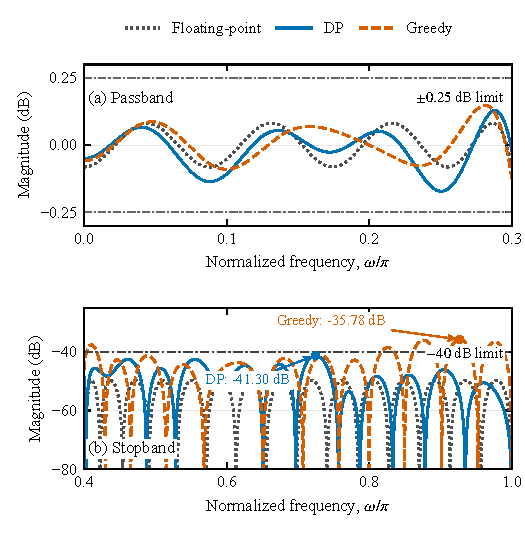
\includegraphics[width=\columnwidth]{figures/frequency_response_quota1.pdf}
\caption{Computed frequency responses of the 48-tap FIR for quota
$[24,16,8]$: (a) passband detail and (b) stopband detail. Gray dash-dot
lines mark the stated limits. DP and greedy stopband peaks are
$-41.30$ and $-35.78$\,dB, respectively. These curves are calculated
from the saved coefficients, not measured on hardware.}
\label{fig:response48}
\end{figure}

Eight RTL variants (DP, greedy, uniform 16-bit, uniform 8-bit; direct
and symmetric-folded) passed XSim simulation over 2,500 cycles with
1,861 valid outputs per design (14,888 total output comparisons) against
an independent 48-term integer-convolution reference. Four
symmetric-folded and direct-form routes were completed on the same
XC7A35T part. Table~\ref{tab:fpga48} reports routed resources for the
DP and greedy symmetric-folded designs.

The tested RTL uses signed 16-bit input samples with 14 fractional bits
and signed coefficient words with one sign bit and $w-1$ fractional bits.
Folded products use a signed 17-bit pair sum. Products and every registered
partial-sum node at tree levels 1--5 are signed 38-bit values with 29
fractional bits; the output is the signed 38-bit value at level 5, also
with 29 fractional bits (9 remaining sign/integer bits). Product alignment
uses exact left shifts, with no rounding or saturation; fixed-width
overflow wraps. The generated vectors remain within the representable
38-bit output range. The eight registered arithmetic stages give a
seven-edge accepted-input to valid-output difference in the testbench.
These statements describe the tested RTL and are not a general resource
model for arbitrary widths.

\begin{table}[!t]
\caption{Forty-eight-tap routed resources for quota $[24,16,8]$}
\label{tab:fpga48}
\centering
\scriptsize
\resizebox{\columnwidth}{!}{%
\begin{tabular}{l r r r r r r}
\toprule
Design & DSP & LUT$_L$ & LUT$_M$ & Slice LUT & FF & Reg--reg (ns)\\
\midrule
DP, folded & 21 & 322 & 32 & 354 & 1066 & 4.344\\
Greedy, folded & 21 & 200 & 16 & 216 & 997 & 5.189\\
DP, direct & 38 & 654 & 80 & 734 & 1106 & 5.763\\
Greedy, direct & 39 & 412 & 64 & 476 & 1043 & 4.879\\
\bottomrule
\end{tabular}}
\vspace{1mm}
\parbox{\columnwidth}{\scriptsize Overall WNS (row order):
$-0.213$, $-0.430$, $-0.435$, $-0.213$\,ns. Negative WNS on assumed
output-delay paths.}
\end{table}

The response-compliant DP allocation uses more slice LUTs (354 vs.\ 216)
and flip-flops (1066 vs.\ 997) than the non-compliant greedy allocation;
this is a bounded resource--response tradeoff for one filter and one
quota, not a general superiority claim. No 48-tap board test, measured
Fmax, sustained throughput, or power measurement was performed.


\section{Robustness Study: Five Filter Specifications}
\label{sec:robustness}

% Robustness study section for tech report

\subsection{Designs and Quotas}

To assess whether the 48-tap base-case observation generalizes, five
FIR designs were tested under three proportional quotas each (15
design/quota combinations). The designs are:

\begin{itemize}
\item A: 48-tap, passband 0--0.3$\pi$, stopband 0.4$\pi$--$\pi$,
$-40$\,dB (base case)
\item B: 48-tap, same bands, $-50$\,dB stopband limit
\item C: 48-tap, passband 0--0.2$\pi$, stopband 0.3$\pi$--$\pi$,
$-40$\,dB (narrower transition)
\item D: 36-tap, same bands and limit as A (replaced the originally
planned 32-tap case, which did not meet $-40$\,dB as a floating-point
prototype)
\item E: 64-tap, same bands and limit as A
\end{itemize}

All five floating-point prototypes satisfy their stated passband and
stopband limits. Quotas are proportional to the 48-tap base case
($[24,16,8]$, $[16,24,8]$, $[12,24,12]$), scaled proportionally to the
tap count and adjusted to sum exactly to that count. Some scaled quotas
are odd (for example, $[22,32,10]$ for 64 taps).

\subsection{Results}

Table~\ref{tab:robust} reports the coefficient SSE and computed stopband
peak for each design/quota/method combination. DP and MILP coefficient-SSE
optima agree in every case.

\begin{table}[!t]
\caption{Robustness study: coefficient SSE and computed stopband peak}
\label{tab:robust}
\centering
\scriptsize
\resizebox{\columnwidth}{!}{%
\begin{tabular}{c l r r c c c}
\toprule
Case & Quota & DP SSE & Greedy SSE & DP stop (dB) & DP pass? & Greedy pass?\\
\midrule
A & $[24,16,8]$ & $1.86\!\cdot\!10^{-5}$ & $6.67\!\cdot\!10^{-5}$ & $-41.30$ & Yes & No\\
A & $[16,24,8]$ & $5.61\!\cdot\!10^{-5}$ & $1.07\!\cdot\!10^{-4}$ & $-35.32$ & No & No\\
A & $[12,24,12]$ & $9.93\!\cdot\!10^{-5}$ & $1.25\!\cdot\!10^{-4}$ & $-31.45$ & No & No\\
B & $[24,16,8]$ & $4.02\!\cdot\!10^{-5}$ & $8.42\!\cdot\!10^{-5}$ & $-35.55$ & No & No\\
B & $[16,24,8]$ & $9.35\!\cdot\!10^{-5}$ & $1.24\!\cdot\!10^{-4}$ & $-34.02$ & No & No\\
B & $[12,24,12]$ & $1.56\!\cdot\!10^{-4}$ & $1.56\!\cdot\!10^{-4}$ & $-32.42$ & No & No\\
C & $[24,16,8]$ & $5.47\!\cdot\!10^{-5}$ & $9.62\!\cdot\!10^{-5}$ & $-34.86$ & No & No\\
C & $[16,24,8]$ & $8.18\!\cdot\!10^{-5}$ & $1.16\!\cdot\!10^{-4}$ & $-35.32$ & No & No\\
C & $[12,24,12]$ & $1.32\!\cdot\!10^{-4}$ & $1.51\!\cdot\!10^{-4}$ & $-31.85$ & No & No\\
D & $[18,12,6]$ & $2.22\!\cdot\!10^{-5}$ & $2.22\!\cdot\!10^{-5}$ & $-35.60$ & No & No\\
D & $[12,18,6]$ & $5.94\!\cdot\!10^{-5}$ & $5.94\!\cdot\!10^{-5}$ & $-30.75$ & No & No\\
D & $[10,16,10]$ & $3.02\!\cdot\!10^{-4}$ & $3.02\!\cdot\!10^{-4}$ & $-28.16$ & No & No\\
E & $[32,22,10]$ & $2.20\!\cdot\!10^{-5}$ & $7.67\!\cdot\!10^{-5}$ & $-40.76$ & Yes & No\\
E & $[22,32,10]$ & $5.50\!\cdot\!10^{-5}$ & $8.08\!\cdot\!10^{-5}$ & $-36.78$ & No & No\\
E & $[16,32,16]$ & $8.68\!\cdot\!10^{-5}$ & $9.68\!\cdot\!10^{-5}$ & $-32.85$ & No & No\\
\bottomrule
\end{tabular}}
\end{table}

\begin{figure*}[!t]
\centering
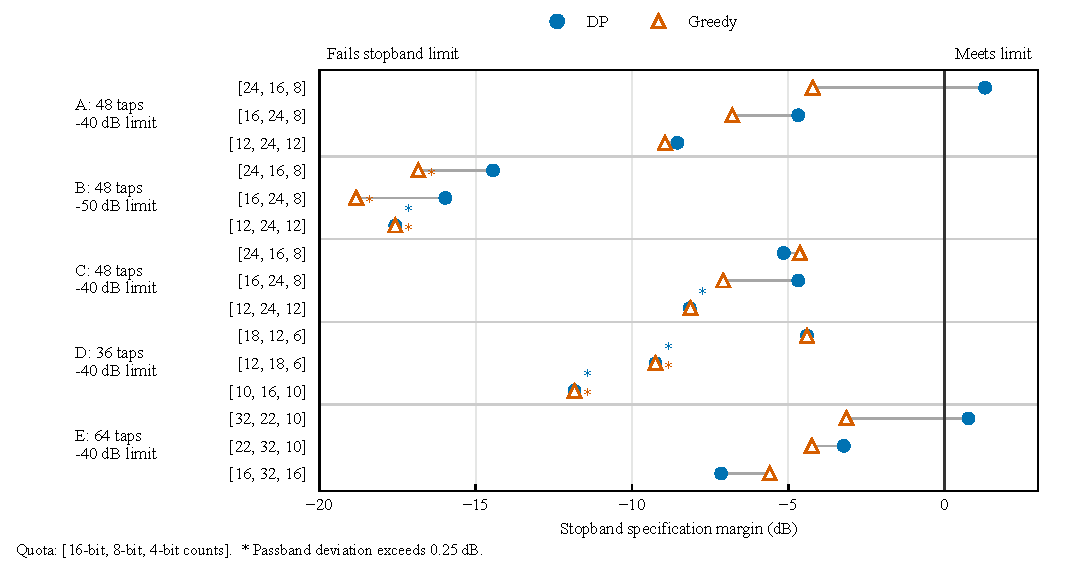
\includegraphics[width=\textwidth]{figures/robustness_margin.pdf}
\caption{All 15 design/quota combinations, using computed responses.
Margin is the specified stopband upper limit minus the computed stopband
peak; nonnegative values meet the stopband limit. Case B uses $-50$\,dB;
the other cases use $-40$\,dB. Asterisks mark passband deviations exceeding
$0.25$\,dB. Hollow greedy triangles keep coincident DP markers visible.
DP meets both limits in 2/15 combinations; greedy in 0/15.
These are software results, not hardware measurements.}
\label{fig:robust-margin}
\end{figure*}

\subsection{Interpretation}

Figure~\ref{fig:robust-margin} shows the stopband margin for every tested
combination and flags passband violations. DP meets both response limits
in 2 of 15 combinations; greedy meets
them in 0. The two DP passes occur for the highest-precision quota in
cases A and E. This is not a universal frequency-response advantage:
in case C's first quota, greedy has a slightly lower stopband peak
($-35.37$ vs.\ $-34.86$\,dB), although both fail the $-40$\,dB limit.

Lower coefficient SSE does not imply lower stopband peak or compliance
with a response specification. These results support a bounded
observation about five prototypes and three proportional quotas only;
they do not establish general performance claims. All results are
software frequency-response calculations; the 36- and 64-tap designs
were not synthesized, routed, or tested on hardware.


\section{Response-Aware Allocation: Feasibility Investigation}
\label{sec:response_aware}

% Response-aware allocation section for tech report

This section documents an investigation into whether the coefficient-SSE
objective could be replaced by a frequency-response-aware objective, and
whether the resulting allocation could be solved exactly under exact
quota constraints.

\subsection{Motivation and Mathematical Structure}

The coefficient-SSE objective $\sum_i e_i^2$ is (by Parseval's theorem)
proportional to the unweighted integrated squared frequency-response
error over the full band. To focus on stopband compliance, the natural
objective is the stopband-weighted integrated squared complex-response
error $\mathbf{e}^\top R \mathbf{e}$, where
\begin{equation}
R_{ij} = \frac{1}{\pi} \int_{\Omega_\text{stop}} \cos(\omega(i-j))\,d\omega
\end{equation}
and $\Omega_\text{stop}$ is the stopband interval.

Three key properties were established:
\begin{enumerate}
\item $R_{ii}$ is the same for all tap positions $i$: the diagonal
weight equals the stopband bandwidth fraction and does not vary with
tap index. Diagonal approximation therefore produces a uniform
scaling of the SSE objective and does not change the allocation.
\item $R$ has nonzero off-diagonal elements (magnitudes $6\times10^{-6}$
to $0.30$ for the 48-tap case), so the objective $\mathbf{e}^\top R
\mathbf{e}$ is not separable in the tap errors $e_i$. The existing
quota DP, which assumes a separable objective, cannot directly solve
the weighted formulation.
\item Fang et al.~\cite{fang2025mixedprecision} also studied FIR
allocation with a frequency-domain objective (minimax), so the
objective type alone does not establish novelty.
\end{enumerate}

\subsection{Small-Scale Exhaustive Screening}

To assess whether handling the cross-terms changes the optimal
allocation, exhaustive search was run on five 8-tap filters under two
quotas each (10 cases). Each case enumerated all feasible assignments
(420--560 per case), found the SSE-minimizing allocation and the
$\mathbf{e}^\top R \mathbf{e}$-minimizing allocation, and compared them.

In 6 of 10 cases, the two optima differed and the weighted-optimal
allocation had a lower stopband peak. However, the absolute stopband
peaks for these 8-tap filters are poor ($-5$ to $-20$\,dB), and the
improvements are small ($0.2$--$1.2$\,dB). The 10 cases arise from 5
filter designs $\times$ 2 quotas; independence is limited.

\subsection{Forty-Eight-Tap MIQP Attempt}

To test whether the weighted objective can be solved exactly at realistic
filter scales, the objective was linearized using binary product
variables. For each pair $(i,k),(j,l)$ with $i<j$, a product variable
$y = x_{i,k} x_{j,l}$ was introduced with standard McCormick
inequalities. The resulting MILP had:
\begin{itemize}
\item 144 width-selection binary variables
\item 10,152 product binary variables
\item 51 equality constraints
\item 30,456 McCormick inequality constraints
\end{itemize}

MATLAB \texttt{intlinprog} was warm-started with the SSE-DP solution.
After approximately 93 seconds, the root-node LP lower bound was
approximately $-5.637 \times 10^{-4}$ against an incumbent of
$7.4603 \times 10^{-6}$ (gap~$\approx 7{,}656\%$), with no
branch-and-bound nodes explored. The run was manually interrupted after
approximately 93 seconds under the pre-declared slow-progress stopping
condition. The root bound changed negligibly from approximately
$-5.6371\times10^{-4}$. Ctrl+C terminated MATLAB before it returned an
exit flag or final allocation. The negative LP bound reflects weak LP
relaxation from the McCormick linearization; it is not a property of the
objective.

\subsection{Summary and Decision}

Under the pre-declared stopping conditions (stop if progress is too slow;
otherwise cap the run at 1 hour), this branch was closed:

\begin{quote}
\textit{STOP: The direct pairwise-product MILP has a weak LP relaxation
that did not certify global optimality in the observed run.
No response-aware allocation or improvement claim follows from the
attempted runs.}
\end{quote}

This outcome does not imply that response-aware allocation with exact
quota constraints is mathematically intractable. A dedicated MIQP solver
(e.g., Gurobi or CPLEX) or a stronger relaxation strategy may
certify global optimality at 48-tap scale. This remains future work
conditioned on solver availability.


\section{Conclusion}
\label{sec:conclusion}

This report evaluated exact-quota mixed-precision FIR quantization as
an instance of unit-capacity transportation. The DP implements a known
cost-constrained optimization principle; no algorithmic novelty is
claimed. Its coefficient-SSE optimum was verified by 29 exhaustive
checks and 108 MILP comparisons (maximum discrepancy
$4.34\times10^{-19}$).

Hardware evidence comprises six routed 8-tap runs and 942 bit-exact
board comparisons, plus four routed 48-tap runs and 14,888 RTL output
comparisons. In the 48-tap base case, DP meets the stopband limit where
same-quota greedy fails, at the cost of more LUTs and registers.
Across five designs and 15 design/quota combinations, DP meets both
response limits in two cases and greedy in none; greedy nevertheless
has a lower stopband peak in some failed cases. Coefficient-SSE
optimality therefore does not guarantee spectral compliance.

The band-weighted response objective contains cross-terms, while its
uniform diagonal approximation leaves the SSE allocation unchanged.
The 48-tap binary-product MILP had a weak root relaxation and was
manually stopped after about 93 seconds under the pre-declared
slow-progress condition. No solver exit flag, final allocation, or
optimality certificate was returned. This observed run does not
establish mathematical intractability.

Future work includes tighter response-aware formulations or dedicated
MIQP solvers, and 48-tap board testing, power measurement, and Fmax
characterization. The released code and data preserve both the positive
validation results and these limitations.


\section*{Code and Data Availability}
The source code, experimental data, FPGA RTL, and test vectors are available at
\url{https://github.com/Bairuirui68/exact-quota-mixed-precision-fir}.

\section*{Acknowledgment}
Codex (OpenAI) assisted with manuscript drafting, code generation,
experiment automation, and verification. The authors are responsible
for checking all claims, data, and citations.

\bibliographystyle{ieeetr}
\bibliography{references}

\end{document}
